\documentclass[10pt]{article}

\usepackage[utf8]{inputenc}
\usepackage{graphicx}
\usepackage{amsmath}
\usepackage{booktabs}
\usepackage{hyperref}
\usepackage{caption}
\usepackage{subcaption}
\usepackage{siunitx}
\usepackage{float}
\usepackage[margin=2.5cm]{geometry}
\usepackage{tikz}
\usetikzlibrary{positioning, arrows.meta}
\usepackage[style=ieee]{biblatex}
\addbibresource{refs.bib}

% Optimisation de l'espacement
\usepackage{titlesec}
\titlespacing*{\section}{0pt}{0.7em}{0.3em}
\titlespacing*{\subsection}{0pt}{0.5em}{0.2em}

% Figures compactes
\captionsetup[figure]{font=small, labelfont=bf, skip=3pt}
\captionsetup[table]{font=small, labelfont=bf, skip=3pt}

\title{Active Control of a Continuum Robot Based on a Sequential Locking Mechanism}
\author{Louis Horak \\ CREATE Lab, EPFL}
\date{\today}

\begin{document}
\maketitle
\clearpage
%------------------------------------------------
\section{Introduction}

Soft continuum robots offer inherent safety and flexibility, making them ideal for applications such as minimally invasive surgery or navigation in complex environments \cite{burgner2015}. However, they often suffer from low payload capacity and imprecise control due to their inherent compliance and complex modeling \cite{walker2013}. To address this trade-off, Wan introduced a hybrid robotic arm design combining a compliant "trimmed helicoid" outer structure with a rigid internal structure \cite{wan2024sequential}.

This internal backbone, the Lockable Spine Mechanism (LSM), utilizes a series of Hirth joints—conical teeth that interlock to prevent rotation. A single tendon actuates these joints. While the tension in the tendon pulls the faces together to ensure mechanical locking, the friction along the tendon path allows the joints to engage sequentially from base to tip \cite{wan2024sequential}. This enables the robot to transition from a flexible state for navigation to a rigid state for load bearing.

However, the original work focused primarily on mechanical validation and open-loop actuation. A significant limitation of the previous prototype is the inability to control multiple curvature configurations in closed-loop. In the unlocked compliant state, the robot remains susceptible to external disturbances and hysteresis. This project aims to bridge this gap by implementing a closed-loop control strategy. By integrating distal IMU sensing and active feedback, we aim to accurately regulate the bending angle $\psi$, which corresponds to rotation about the yaw axis of the distal IMU (hence labeled "Yaw" in all experimental plots), and maintain a desired configuration, effectively using a sequence of single curvatures to achieve complex multi-curvature shapes despite sensing constraints.

\begin{figure}[H]
    \centering
    \begin{subfigure}[t]{0.49\linewidth}
        \centering
        \includegraphics[height=8.5cm, width=\linewidth, keepaspectratio]{Wang_design.png}
        \caption{Sequential locking mechanism.}
        \label{fig:locking_principle}
    \end{subfigure}
    \hfill
    \begin{subfigure}[t]{0.49\linewidth}
        \centering
        \includegraphics[height=8.5cm, width=\linewidth, keepaspectratio]{Systeme_angle.png}
        \caption{Angle convention.}
        \label{fig:angle_convention}
    \end{subfigure}
    \caption{(a) Principle of the sequential locking mechanism. (b) Angle convention for bending and yaw.}
    \label{fig:system_overview}
\end{figure}

%------------------------------------------------
\section{Methods}

\subsection{State Estimation Strategy}
The initial control strategy aimed to utilize the four optical encoders at each joint to determine multiple curvatures. However, their coarse resolution (\SI{3.75}{\degree}) and significant quantization noise made smooth feedback control impossible. While the integration of absolute PHS11 analog potentiometers was planned to resolve this, hardware delivery delays necessitated an alternative approach using the distal IMU.

To achieve multi-curvature shapes despite these constraints, a sequential control and locking strategy was implemented. The system relies on a proportional relationship between the global distal yaw $\psi$—measured by the IMU's local yaw axis and corresponding to the global bending angle—and the individual joint angles $\theta_i$: $\theta_i \approx K_i \cdot \psi$. This relationship was empirically validated through controlled bending cycles, correlating discrete encoder steps with high-resolution IMU data. An automated calibration tool sweeps the arm through its range of motion ($\pm$30°) using ramped velocity profiles to minimize inertial artifacts. A linear regression identified the coefficients $K_i$, allowing for continuous estimation of the robot's configuration.

The control process operates as follows (Fig.~\ref{fig:sequential_process}):

\begin{figure}[H]
\centering
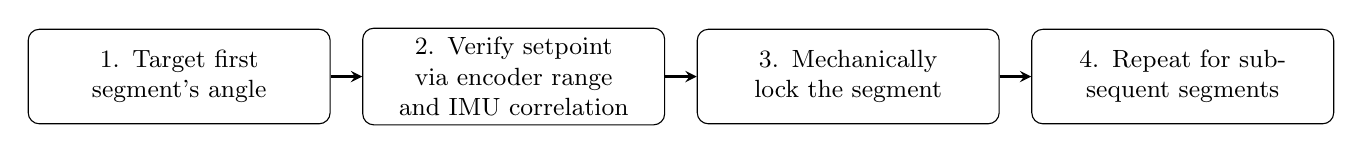
\begin{tikzpicture}[
    node distance=0.4cm,
    block/.style={rectangle, draw, rounded corners, text width=3.6cm, minimum height=1.2cm, text centered, font=\small},
    arrow/.style={->, >=stealth, thick}
]

% Nodes disposés horizontalement
\node[block] (step1) {1. Target first segment's angle};
\node[block, right=of step1] (step2) {2. Verify setpoint via encoder range and IMU correlation};
\node[block, right=of step2] (step3) {3. Mechanically lock the segment};
\node[block, right=of step3] (step4) {4. Repeat for subsequent segments};

% Arrows
\draw[arrow] (step1) -- (step2);
\draw[arrow] (step2) -- (step3);
\draw[arrow] (step3) -- (step4);

\end{tikzpicture}
\caption{Sequential control and locking process for multi-curvature shapes.}
\label{fig:sequential_process}
\end{figure}

The calibration yielded the following coefficients:
\begin{equation*}
    K_1 = -0.131, \quad K_2 = -0.328, \quad K_3 = -0.337, \quad K_4 = -0.198
\end{equation*}

\subsection{System Identification}
A frequency-domain analysis was performed using a chirp excitation signal (\SI{0.1}{rad/s} to \SI{3}{rad/s}). The open-loop transfer function relates the differential velocity command $u$ to the distal yaw $\psi$.

To ensure signal quality, raw IMU data were processed through a median filter to remove impulsive noise spikes. This filter introduces a frequency-dependent phase delay. This lag was modeled and mathematically included in our best-fit algorithm to estimate the transfer function. The Bode plot (Fig.~\ref{fig:bode_analysis}) confirms the integrating behavior of $H(s)$. The phase response includes the explicitly modeled delay from the median filter (window size $k=5$), which was taken into account in the controller stability analysis.

The resulting Bode analysis (Fig.~\ref{fig:bode_analysis}) yielded the transfer function:
\begin{equation}
    H(s) = \frac{-14.72}{s^{2} + 4.574s}
\end{equation}

Transfer function parameters were estimated via least-squares optimization on the frequency-domain data using a custom pole-zero fitting tool.

\begin{figure}[H]
    \centering
    \includegraphics[width=\linewidth]{BODE_DIAGRAM.png}
    \caption{Bode plot of identified transfer function $H(s)$.}
    \label{fig:bode_analysis}
\end{figure}

\subsection{Controller Design and Stability Analysis}
\label{sec:controller_design}
A proportional controller computes the velocity command: $u(t) = K_p (\psi_{\text{target}} - \psi_{\text{measured}})$. The negative sign of the plant $H(s)$ requires $K_p < 0$ for correct feedback polarity. The middle plot in Fig.~\ref{fig:step_response} shows the control signal $u$ in \si{rad/s} (velocity command to motors).

Despite its simplicity, a P-controller was found to be sufficient for several reasons. First, the plant $H(s)$ exhibits inherent integrating behavior (as seen in its transfer function), which theoretically ensures zero steady-state error for step inputs without the need for an integral (I) term. Second, the Dynamixel XC330 motors feature an internal hardware PID loop for velocity and position control; this low-level regulation likely contributes to the system's high stability and performance, rendering additional derivative (D) action in the high-level controller unnecessary.

\paragraph{Stability and Delay Compensation}
The median filter (window size $k=5$, sampling frequency $f_s = \SI{50}{Hz}$) introduces a delay $\tau = \frac{k-1}{2f_s} \approx \SI{0.04}{s}$. Using a first-order approximation ($e^{-\tau s} \approx 1 - \tau s$), the closed-loop characteristic equation becomes:
\begin{equation}
    s^{2} + (B + A K_p \tau)s - A K_p = 0
\end{equation}
where $A=14.72$ and $B=4.574$. Stability requires $B + A K_p \tau > 0$. With $K_p = -0.5$, the system remains stable with a predicted damping ratio $\zeta \approx 0.79$, ensuring a fast response with minimal overshoot.

\subsection{Automated Performance Testing}
A comprehensive GUI was developed to automate testing and data collection. The interface provides:
\begin{itemize}
    \item Real-time plotting of yaw, control signal, and motor currents
    \item Automated step response and disturbance rejection tests
    \item Parameter adjustment and calibration procedures
    \item CSV export of all test data for analysis
\end{itemize}
This interface enabled efficient parameter tuning and real-time monitoring during experiments.

%------------------------------------------------
\section{Experimental Setup}

\subsection{Hardware Configuration}
The continuum arm is actuated by two Dynamixel XC330 motors in a differential tendon configuration. The sensing system comprises:
\begin{itemize}
    \item \textbf{Global orientation}: BNO055 IMU mounted at the distal end
    \item \textbf{Joint angles}: 4× optical encoders with \SI{3.75}{\degree} resolution
    \item \textbf{Control interface}: U2D2 for Dynamixel communication, FTDI for IMU
\end{itemize}

\subsection{Software Implementation}
The control loop runs at \SI{50}{Hz} in Python, with separate threads for sensor reading, motor control, and GUI updates. The median filter operates with a 5-sample window to reject noise spikes while minimizing phase delay.

\subsection{Automated Calibration}
The calibration procedure utilizes a velocity-ramped profile to minimize inertial effects. By sweeping the arm from \SI{0}{\degree} to \SI{30}{\degree} to \SI{-30}{\degree} and back while logging IMU yaw and encoder counts, the system identifies the $K_i$ coefficients via least-squares regression. This ensures the estimation is robust to variations in tendon tension.

%------------------------------------------------
\section{Results}

\subsection{Step Response Performance}
Figure~\ref{fig:step_response} shows the system's response to a \SI{20}{\degree} step command. The top plot displays the measured bending angle $\psi$ (labeled \textit{Yaw} per IMU convention), demonstrating accurate tracking. The middle plot shows the control signal $u$ in \si{rad/s}, and the bottom plot shows motor currents, which reflect the control effort required.

The response shows a rise time of \SI{1.07}{s} and a settling time of \SI{1.67}{s}. The steady-state error is \SI{-0.11}{\degree}, demonstrating the effectiveness of the proportional controller combined with the system's integrating dynamics.

\begin{table}[H]
\centering
\small
\begin{tabular}{@{}lccc@{}}
\toprule
Metric & Theory ($\zeta=0.79$) & Experimental & Error \\ \midrule
Rise Time $t_r$ & \SI{0.92}{s} & \SI{1.07}{s} & 16.3\% \\
Settling Time $t_s$ & \SI{1.45}{s} & \SI{1.67}{s} & 15.2\% \\
Overshoot $M_p$ & \SI{1.9}{\%} & \SI{0.65}{\%} & -65.8\% \\ \bottomrule
\end{tabular}
\caption{Comparison of predicted and experimental dynamic characteristics. Values represent a typical run from a series of consistent trials with low standard deviation. The theoretical values are derived from the identified model with $K_p=-0.5$.}
\label{tab:results}
\end{table}

\begin{figure}[H]
    \centering
    \includegraphics[width=0.9\linewidth]{performance_test_step_response_20251220_104005.png}
    \caption{Step response to \SI{20}{\degree} command: bending angle (Yaw), control signal, and motor currents.}
    \label{fig:step_response}
\end{figure}

\subsection{Active Disturbance Rejection}
Figure~\ref{fig:disturbance_response} illustrates active disturbance rejection at \SI{-45}{\degree}. The transient between $t=0$ and $t=4$s corresponds to manual placement of a \SI{1}{kg} load. During this interval, the recorded deviation is due to the manual handling of the arm. Once released, the controller immediately compensates for the load, returning the system to the setpoint in approximately \SI{1.5}{s}. The Dynamixel motors effectively absorb the external tension, providing "active stiffness" to the compliant structure.

\begin{figure}[H]
    \centering
    \includegraphics[width=0.9\linewidth]{performance_test_disturbance_rejection_20251220_104005.png}
    \caption{Disturbance rejection at \SI{-45}{\degree} under \SI{1}{kg} load.}
    \label{fig:disturbance_response}
\end{figure}

%------------------------------------------------
\section{Discussion \& Conclusion}

The results validate that a simple proportional controller is sufficient to stabilize the integrating dynamics of the tendon-driven system. The disturbance rejection test proves that active control can serve as a functional substitute for mechanical locking during dynamic phases, providing "active stiffness" through continuous feedback compensation.

\subsection{Integration with Sequential Locking}
The calibrated $K_i$ coefficients serve a dual purpose: they enable state estimation for control and provide the kinematic mapping needed for sequential locking. When a segment is locked, the corresponding $K_i$ effectively becomes 0, and the control law can be adjusted accordingly. This provides a straightforward pathway for integrating active control with mechanical locking operations.

\subsection{Limitations and Future Improvements}
The $K_i$-based estimation assumes uniform bending, which may not hold under complex loads. The immediate path to improvement is the integration of PHS11 analog potentiometers. These absolute sensors will provide continuous joint-angle measurements, eliminating the proportional assumption and enhancing precision. Future work includes:
\begin{itemize}
    \item Implementing sequential locking control using the calibrated $K_i$ coefficients
    \item Extending control to 3D using full IMU orientation
    \item Exploring adaptive control strategies for varying locking states
\end{itemize}

\subsection{Conclusion}
This work successfully transitions the hybrid continuum robot from a mechanical prototype to a controlled system. The calibrated $K_i$ coefficients now serve as a bridge between continuous active control and discrete sequential locking states, enabling precise configuration control while maintaining compliance advantages. The system achieves sub-degree accuracy, rapid response, and effective disturbance rejection, validating the approach for hybrid continuum robot control.

%------------------------------------------------
\printbibliography

\appendix
\newpage
\section*{Appendix: Code and CAD Resources}

\subsection*{Source Code}
All Python source code is available on the CREATE Lab GitHub repository. The following files comprise the complete control system:

\begin{itemize}
    \item \textbf{MotorWidebandID.py} (579 lines) -- System identification via chirp excitation and cross-spectral density analysis
    \item \textbf{SequentialJointCalibration.py} (960 lines) -- Automated $K_i$ coefficient calibration with velocity-ramped profiles
    \item \textbf{TransferFunctionEstimator.py} (428 lines) -- Frequency-domain transfer function fitting via least-squares optimization
    \item \textbf{robot\_performance\_tests.py} (1314 lines) -- Comprehensive testing framework for step response and disturbance rejection
    \item \textbf{dynamixel\_controller.py} (474 lines) -- Hardware abstraction layer for Dynamixel motor control and IMU interfacing
\end{itemize}

Repository access: Contact Kai Huang or refer to the CREATE Lab GitHub page for full code repository and documentation.

\subsection*{CAD Components}
The complete mechanical design is available in Autodesk Fusion 360 format. All CAD files and components are packaged in the file \texttt{ASSEMBLAGE.f3z}.

The assembly file is located in the CREATE Lab Fusion 360 workspace at: \texttt{Soft\_Sensors\_and\_bodies > Louis\_Horak > ASSEMBLAGE.f3z}. The file imports all custom components created for this project.



\end{document}
